              
                %%%%%%%%%%%%%%%%%%%%%%%%%%%%%%%%%%%%%%%%%%%%%%%%%%%%%%%%%%%%%%%%%%%%%%
% LaTeX Example: Project Report
%
% Source: http://www.howtotex.com
%
% Feel free to distribute this example, but please keep the referral
% to howtotex.com
% Date: March 2011 
% 
%%%%%%%%%%%%%%%%%%%%%%%%%%%%%%%%%%%%%%%%%%%%%%%%%%%%%%%%%%%%%%%%%%%%%%
% How to use writeLaTeX: 
%
% You edit the source code here on the left, and the preview on the
% right shows you the result within a few seconds.
%
% Bookmark this page and share the URL with your co-authors. They can
% edit at the same time!
%
% You can upload figures, bibliographies, custom classes and
% styles using the files menu.
%
% If you're new to LaTeX, the wikibook is a great place to start:
% http://en.wikibooks.org/wiki/LaTeX
%
%%%%%%%%%%%%%%%%%%%%%%%%%%%%%%%%%%%%%%%%%%%%%%%%%%%%%%%%%%%%%%%%%%%%%%
% Edit the title below to update the display in My Documents
%\title{Project Report}
%
%%% Preamble
\documentclass[paper=letter, fontsize=11pt]{scrartcl}
\usepackage{url}
\usepackage{color}
\usepackage{fourier}
\usepackage{listings}
\usepackage[T1]{fontenc}
\usepackage[english]{babel}
\usepackage[pdftex]{graphicx}
\usepackage[margin=2.5cm]{geometry}
\usepackage{amsmath,amsfonts,amsthm} % Math packages
                                       % English language/hyphenation
\usepackage[protrusion=true,expansion=true]{microtype}  

%%% Maketitle metadata
\newcommand{\horrule}[1]{\rule{\linewidth}{#1}}     % Horizontal rule

\title{
        %\vspace{-1in}  
        \usefont{OT1}{bch}{b}{n}
        \normalfont \normalsize \textsc{Universidad de los Andes, Departamento de F\'isica \\
        F\'isica at\'omica} \\ [25pt]
        \horrule{0.5pt} \\[0.4cm]
        \huge Pozo finito de potencial \\
        \horrule{2pt} \\[0.5cm]
}
\author{
        \normalfont                                 \normalsize
        Juan Barbosa, 201325901\\[-3pt]      \normalsize
        Febrero 16, 2017
}
\date{}

\lstset{keywordstyle=\color{blue}, basicstyle=\scriptsize, frame=single, language=Python}

%%% Begin document
\begin{document}
\maketitle

\[
\boxed{-\dfrac{\hbar^2}{2m}\nabla^2\Psi(x) + V(x)\Psi(x) = E\Psi(x)}
\]

Para el caso del potencial finito la ecuaci\'on de Schr\"odinger se aplica a las tres regiones de interes. Para las regiones con potencial $V_0 > E$ la soluci\'on a la funci\'on de onda $\Psi$ ser\'a:
\begin{equation}
	\Psi_{I}(x) = Ae^{kx} + Be^{-kx} \qquad , \qquad k = \sqrt{\dfrac{2m(V_0-E)}{\hbar^2}}
\end{equation}

Teniendo en cuenta que la funci\'on debe ser acotada para la regi\'on $I$ la funci\'on $\Psi(x)$ debe anularse para $x = -\infty$, lo anterior implica que $B = 0$. Para la regi\'on $III$ se usa un argumento an\'alogo con lo cual se obtiene:
\begin{equation}
	\begin{array}{c}
		\Psi_{I}(x) = Ae^{kx} \\
		\Psi_{III}(x) = Ce^{-kx}
	\end{array}
\end{equation}

En la regi\'on $II$ la soluci\'on es oscilante.

\begin{equation}
	\Psi_{II}(x) = Fe^{i\kappa x} + Ge^{-i\kappa x} \qquad , \qquad \kappa = \sqrt{\dfrac{2mE}{\hbar^2}}
\end{equation}

Usando el m\'etodo de Euler para resolver num\'ericamente se obtiene:
\begin{equation}
	\begin{matrix}
	\dot{\Psi}_n = \dot{\Psi}_{n-1} + \ddot{\Psi}_{n-1}\Delta x \\
	\Psi_n = \Psi_{n-1} + \dot{\Psi}_n\Delta x
	\end{matrix}
	\qquad \text{donde} \qquad \ddot{\Psi} = \dfrac{2m(V_0 - E)}{\hbar^2}\Psi
\end{equation}

El sistema de ecuaciones diferenciales es resuelto usando $N = 1001$ puntos, $dx = 0.003$, $L = 2$ y un potencial $V_0 = 100$. Las unidades usadas son arbitrarias tales que $\hbar^2 =  2m =1$.

\newpage
\lstinputlisting{Schrodinger.py}
\begin{center}
	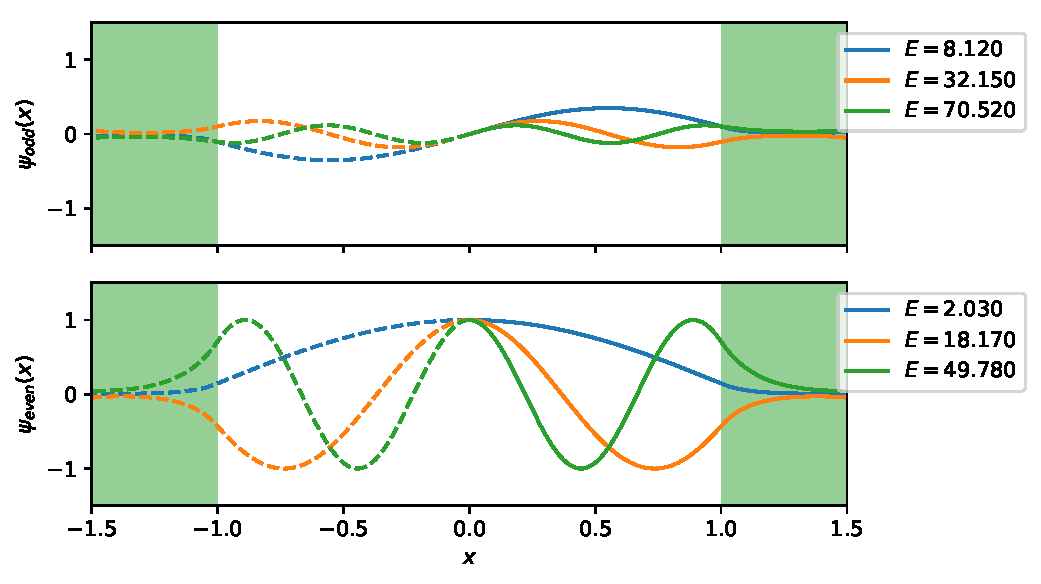
\includegraphics[width=\linewidth]{finite-box.pdf}
\end{center}
\begin{center}
	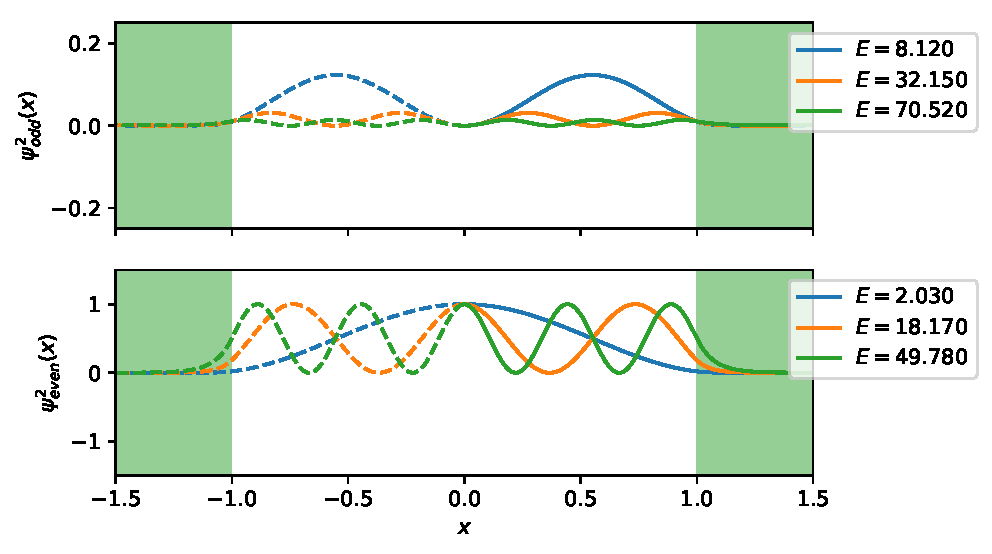
\includegraphics[width=\linewidth]{psi-squared.pdf}
\end{center}

La energ\'ia depende del cuadrado de $n$ como n\'umero cu\'antico. Resultado an\'alogo al de un pozo de potencial infinito. La soluci\'on anal\'itica a la ecuaci\'on es de la forma:
\begin{equation}
\begin{array}{c}
k_{even} = \kappa\tan\dfrac{\kappa L}{2} = \sqrt{\beta^2 - \kappa^2} \\
k_{odd} = -\dfrac{\kappa}{\tan\frac{\kappa L}{2}} = \sqrt{\beta^2 - \kappa^2}\\
\end{array}
\end{equation}
\begin{equation}
\begin{array}{c}
\Psi_{II_{even}}(x) = F\cos(\kappa x)\\
\Psi_{II_{odd}}(x) = F\sin(\kappa x)
\end{array}
\end{equation}

\begin{center}
	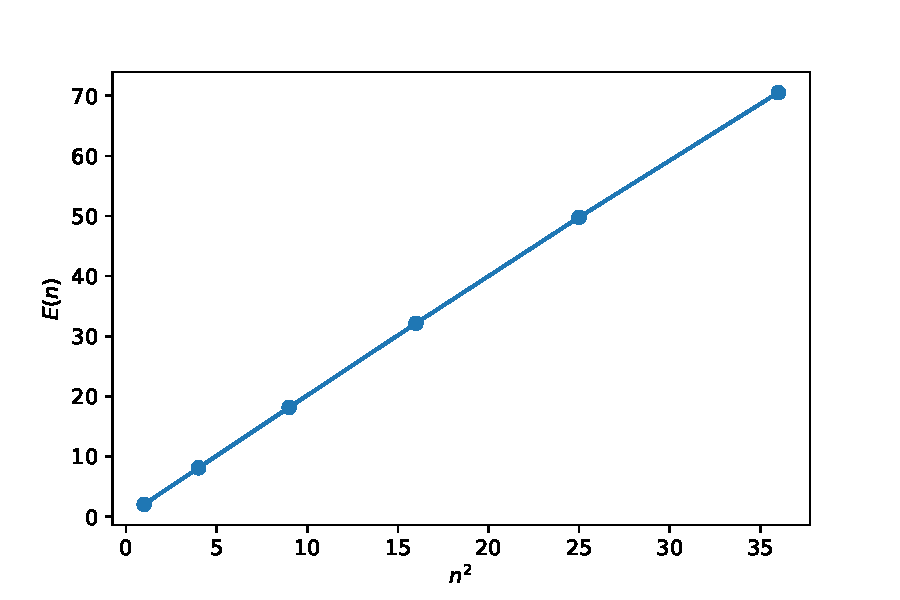
\includegraphics[width=0.5\linewidth]{energy.pdf}
\end{center}
\begin{table}[h]
	\centering
	\begin{tabular}{cc}
		\hline
		$n$ & E \\
		\hline
		1 & 2.030 \\
		2 & 8.120 \\
		3 & 18.170 \\
		4 & 32.150 \\
		5 & 49.780 \\
		6 & 70.520 \\
		\hline
	\end{tabular}
\end{table}

Finalmente para el caso con $E > V_0$ se obtienen soluciones oscilantes para toda regi\'on del espacio. Para las regiones con $V = V_0$ la amplitud se ve reforzada.
\begin{center}
	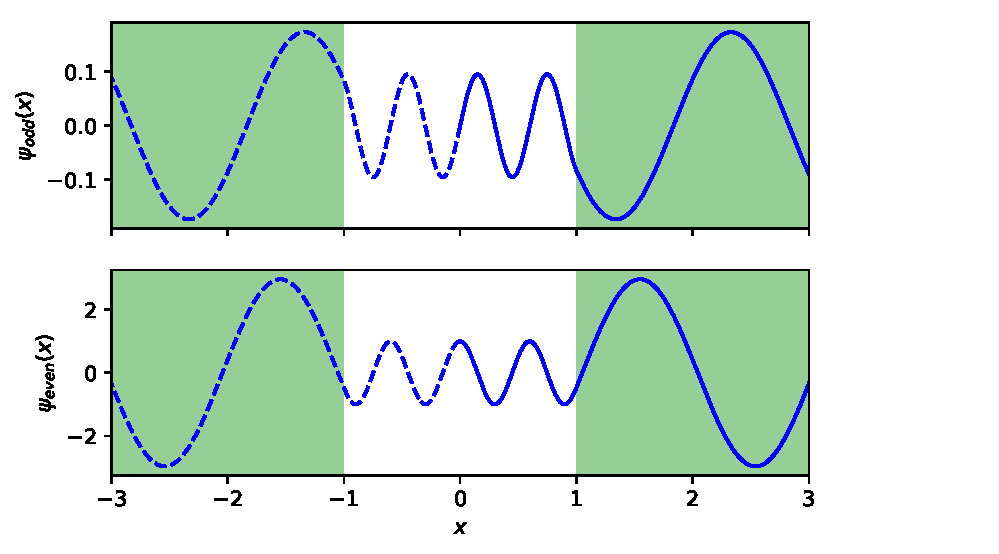
\includegraphics[width=\linewidth]{greater.pdf}
\end{center}
\end{document}
              